\documentclass[c]{beamer}

\usepackage{graphicx}
\usepackage{epsfig}
\usepackage{hyperref}
\usepackage{booktabs, caption}
\usepackage{anyfontsize}

% suppress navigation bar
\beamertemplatenavigationsymbolsempty

\mode<presentation>
{
  \usetheme{jd}
  \setbeamercovered{transparent}
  \setbeamertemplate{items}[circle]
}

% set fonts
\usepackage{fontspec}
\setsansfont{Changa One}
%\setmainfont{Fontin}
\setbeamerfont{frametitle}{size=\LARGE,series=\bfseries}

\usepackage{setspace}
\setstretch{3}
\parindent 0pt

% color definitions
\usepackage{color}
\definecolor{uipoppy}{RGB}{225, 64, 5}
\definecolor{uipaleblue}{RGB}{96,123,139}
\definecolor{uiblack}{RGB}{0, 0, 0}
\definecolor{uigreen}{RGB}{96, 147, 115}
\definecolor{uigreen_dark}{RGB}{31, 39, 42}
\definecolor{uigray}{RGB}{217, 217, 217}
\definecolor{uired}{RGB}{187, 114, 101}

% caption styling
\DeclareCaptionFont{uiblack}{\color{uiblack}}
\DeclareCaptionFont{uipoppy}{\color{uipoppy}}
\captionsetup{labelfont={uipoppy},textfont=uiblack}

% itemize style
\setbeamertemplate{itemize item}{\Huge\raise2.55pt\hbox{\donotcoloroutermaths\cred{$\blacktriangleright$}}}

% see the macros.tex file for definitions
% This program can be redistributed and/or modified under the terms
% of the GNU Public License, version 3.

% adds reference to bottom right of corner of a slide
\usepackage[absolute,overlay]{textpos} % text references in slide corners
\newcommand\textref[1]{%
  \begin{textblock*}{\paperwidth}(0pt,0.99\textheight)
  \raggedleft \tiny{\emph{#1}}\hspace{.5em}
  \end{textblock*}}

% for drawing circles around numbers
% ex. \circled{1} Add some text here.
\usepackage{tikz}
\usepackage{ifthen}
\usetikzlibrary{arrows}
\usetikzlibrary{matrix}
\usetikzlibrary{decorations,arrows}
\usetikzlibrary{decorations.pathmorphing}
\usepgflibrary{decorations.pathreplacing}
\usetikzlibrary{decorations.pathreplacing}


\newcommand*\circled[1]{\tikz[baseline=(char.base)]{
            \node[shape=circle,draw,inner sep=2pt] (char) {#1};}}

% Font sizes
\newcommand{\fontHeadI}[1]{
    \textbf{
      {\fontsize{70}{60}\selectfont #1}
    }
}

\newcommand{\fontHeadII}[1]{
    \textbf{
      {\fontsize{60}{10}\selectfont #1}
    }
}

\newcommand{\fontHeadIII}[1]{
    \textbf{
      {\fontsize{40}{14}\selectfont #1}
    }
}

\newcommand{\fontHeadIV}[1]{
    \textbf{
      {\fontsize{30}{10}\selectfont #1}
    }
}

\newcommand{\fontSmall}[1]{
    {\small #1}
}

% Font color
\newcommand{\cdark}[1]{
  \textcolor{uigreen_dark}{#1}
}

\newcommand{\cgray}[1]{
  \textcolor{uigray}{#1}
}

\newcommand{\cred}[1]{
  \textcolor{uired}{#1}
}

% title slide definition
\title{Git - Eine Einführung}
\author{Jens Dieskau}

\date{\today}

\begin{document}

%--------------------------------------------------------------------
%                           Titelseite
%--------------------------------------------------------------------

\section{Titelseite}

\setbeamercolor{background canvas}{bg=uigreen}
\setbeamertemplate{footline}[default]

\begin{frame}
 \begin{center}
   \fontHeadI{\cgray{Git}} \\
   \fontHeadIII{\cdark{Eine Einführung}} \\
  \end{center}
\end{frame}

%-------------------------------------------------------------------
%                              Datentypen
%-------------------------------------------------------------------
%
\setbeamertemplate{footline}[jdtheme]


\setbeamercolor{background canvas}{bg=uigreen_dark}
\section{Datentypen}
\begin{frame}
 \begin{center}
   \fontHeadII{\cred{Datentypen}}
  \end{center}
\end{frame}

\setbeamercolor{background canvas}{bg=uigreen}
\begin{frame}
  \begin{center}
   \fontHeadIII{\cdark{
     %\hspace{2.5em}blob \\
     %\hspace{2.5em} tree \\
     %\hspace{2.5em} tag \\
     %\hspace{2.5em} commit \\
     blob\\
     tree\\
     tag\\
     commit\\
   }}
 \end{center}
\end{frame}

%\setbeamercolor{background canvas}{bg=uigreen}
%\begin{frame}[t]
%   %\fontHeadIII{\cdark{
%   \begin{itemize}
%     %\setlength{\itemindent}{5em}
%     %\fontHeadIII{\cdark{
%       \item blob
%       \item tree
%       \item commit
%       \item tag
%    % }}
%   \end{itemize}
%  %}}
%\end{frame}

\setbeamercolor{background canvas}{bg=uigreen}
\begin{frame}
 \begin{center}
   \fontHeadI{\cdark{blob}} \\
   \fontHeadIV{\cgray{jede Datei im Repo}}
  \end{center}
\end{frame}

\setbeamercolor{background canvas}{bg=uigreen}
\begin{frame}
 \begin{center}
   \fontHeadI{\cdark{tree}} \\
   \fontHeadIV{\cgray{jedes Verzeichnis}} \\
   \fontSmall{\cgray{(tree-Objekte können andere tree-Objekte und blobs enthalten)}}
  \end{center}
\end{frame}

\setbeamercolor{background canvas}{bg=uigreen}
\begin{frame}
 \begin{center}
   \fontHeadI{\cdark{commit}} \\
   \fontHeadIV{\cgray{Abbild eines tree}} \\
   \fontSmall{\cgray{(zu einer bestimmten Zeit + Metainformationen)}}
  \end{center}
\end{frame}


%-------------------------------------------------------------------
%                              Repository
%-------------------------------------------------------------------
%
\setbeamercolor{background canvas}{bg=uigreen_dark}
\section{Was ist ein Repo?}
\begin{frame}
  \begin{center}
    \fontHeadII{\cred{Repo?}}
  \end{center}
\end{frame}

\setbeamercolor{background canvas}{bg=uigreen}
\begin{frame}
  \begin{center}
    \fontHeadIII{\cdark{
      Repo \\
      Repository \\
    }}
    \vspace{3em}
    \fontHeadIV{\cgray{
      'Aufbewahrungsort' \\
    }}
  \end{center}
\end{frame}

\setbeamercolor{background canvas}{bg=uigreen}
\begin{frame}[t]
  \begin{center}
    \fontHeadIV{\cdark{Graph aus Commits}}
  \end{center}
   \vspace{-\baselineskip}
  \begin{columns}[t]
    \column{1.5cm}
    
    %\begin{block}{}
    
  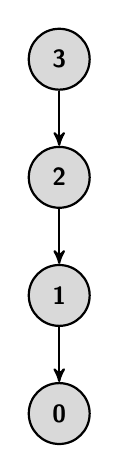
\begin{tikzpicture}[<-,>=stealth',node distance=1.5cm,
    thick,main node/.style={circle,fill=uigray,draw,font=\sffamily\small\bfseries,inner sep=0pt,minimum size=22pt}]
    \node[main node] (0)              {0};
    \node[main node] (1) [above of=0] {1};
    \node[main node] (2) [above of=1] {2};
    \node[main node] (3) [above of=2] {3};

    \path[every node/.style={font=\sffamily\small}]
      \foreach \y [count=\i] in {0,1,2} {
        (\y) edge node {} (\i)
      } ;
  \end{tikzpicture}
    %\end{block}
    \column{4.5cm}
    
    %\begin{block}{}
        \vspace{0.15cm}
        \circled{1}$\textemdash$bastn\"{a}site \\
        \circled{2}$\textemdash${monazite} \\\circled{2}$\textemdash${monazite} \\\circled{2}$\textemdash${monazite} \\\circled{2}$\textemdash${monazite} \\\circled{2}$\textemdash${monazite} \\
        
        
        
        
        
        
        
        
        
        
        
        
        
        
        
        
        
        
        
        
        
        
        
    %\end{block}
  \end{columns}



\end{frame}



\end{document}
